\documentclass[paper=letter, fontsize=11pt]{scrartcl} 
\usepackage{graphicx}
\usepackage{verbatim}
\usepackage{pictex}  
\usepackage{multimedia}
\usepackage{listings}
\usepackage{xcolor,colortbl}
\usepackage[utf8]{inputenc}		%para identificar acentos(encoding)
\usepackage{url}
\usepackage[spanish]{babel} % language/hyphenation
\usepackage{amsmath,amsfonts,amsthm} % Math packages
\usepackage{amsbsy}
\usepackage{amssymb}
\usepackage{fancyvrb}
\usepackage{sectsty} % Allows customizing section commands
\allsectionsfont{\centering \normalfont\scshape} % Make all sections centered, the default font and small caps
\usepackage{float}%para fijar las figuras y tablas
\usepackage{placeins}%fija espacios
\usepackage{fancyhdr} % Custom headers and footers
\pagestyle{fancyplain} % Makes all pages in the document conform to the custom headers and footers
\fancyhead{} % No page header - if you want one, create it in the same way as the footers below
\fancyfoot[L]{} % Empty left footer
\fancyfoot[C]{} % Empty center footer
\fancyfoot[R]{\thepage} % Page numbering for right footer
\renewcommand{\headrulewidth}{0pt} % Remove header underlines
\renewcommand{\footrulewidth}{0pt} % Remove footer underlines
\setlength{\headheight}{13.6pt} % Customize the height of the header

\numberwithin{equation}{section} % Number equations within sections (i.e. 1.1, 1.2, 2.1, 2.2 instead of 1, 2, 3, 4)
\numberwithin{figure}{section} % Number figures within sections (i.e. 1.1, 1.2, 2.1, 2.2 instead of 1, 2, 3, 4)
\numberwithin{table}{section} % Number tables within sections (i.e. 1.1, 1.2, 2.1, 2.2 instead of 1, 2, 3, 4)

\setlength\parindent{0pt} % Removes all indentation from paragraphs - comment this line for an assignment with lots of text

\newcommand{\horrule}[1]{\rule{\linewidth}{#1}} % Create horizontal rule command with 1 argument of height

\title{	
\normalfont \normalsize 
\textsc{Centro de Investigaci\'on en Matem\'aticas (CIMAT). Unidad Monterrey} 
\\ [25pt] 
\horrule{0.5pt} \\[0.4cm] % Thin top horizontal rule
\huge Temas Selectos de Análisis de Datos Complejos (Tarea 4) \\ 
\horrule{2pt} \\[0.5cm] % Thick bottom horizontal rule
}

\author{José Antonio García Ramírez} % Your name

\date{\normalsize\today} % Today's date or a custom date

\begin{document}
\lstdefinestyle{customc}{
  belowcaptionskip=1\baselineskip,
  basicstyle=\footnotesize, 
  frame=lrtb,
  breaklines=true,
  %frame=L,
  %xleftmargin=\parindent,
  language=C,
  showstringspaces=false,
  basicstyle=\footnotesize\ttfamily,
  keywordstyle=\bfseries\color{green!40!black},
  commentstyle=\itshape\color{red!40!black},
  identifierstyle=\color{blue},
  stringstyle=\color{purple},
}

\lstset{breakatwhitespace=true,
  basicstyle=\footnotesize, 
  commentstyle=\color{green},
  keywordstyle=\color{blue},
  stringstyle=\color{purple},
  language=C++,
  columns=fullflexible,
  keepspaces=true,
  breaklines=true,
  tabsize=3, 
  showstringspaces=false,
  extendedchars=true}

\lstset{ %
  language=R,    
  basicstyle=\footnotesize, 
  numbers=left,             
  numberstyle=\tiny\color{gray}, 
  stepnumber=1,              
  numbersep=5pt,             
  backgroundcolor=\color{white},
  showspaces=false,             
  showstringspaces=false,       
  showtabs=false,               
  frame=single,                 
  rulecolor=\color{black},      
  tabsize=2,                  
  captionpos=b,               
  breaklines=true,            
  breakatwhitespace=false,    
  title=\lstname,             
  keywordstyle=\color{blue},  
  commentstyle=\color{dkgreen},
  stringstyle=\color{mauve},   
  morekeywords={\%*\%,...}         
} 


\maketitle % Print the title

\section{Ejercicio 1}


\begin{enumerate}
\item Considera el conjunto de datos Paraná de la libreria \verb|geoR| (\verb|data(parana)|, \verb|help(parana)|)
  \begin{enumerate}
  \item ¿Qué preguntas científicas son interesantes de contestar? ¿Incluyen estimación, predicción o pruebas de hipótesis? \\
  
  Después de recurrir a la documentación del conjunto de datos de Paraná, encontramos que los datos se refieren a la precipitación promedio de la estación seca (mayo a junio) de varios años en el estado de Paraná (Brasil).\\

La primer pregunta interesante se refiere al diseño de recolección de la muestra, si la muestra de registros que se tienen representa una muestra apropiada espacialmente, es decir si es uniforme y toda la superficie de estudio se encuentra representada. En la documentación se refiere a que se cuenta con 143 observaciones que registran 143 estaciones localizadas en todo el estado de Paraná. Si bien en la figura 1.1 (izquierda) podemos apreciar que las estaciones se distribuyen a lo largo de todo el estado desconocemos varios hechos como la fecha de las lecturas (para identificar lecturas del mismo año) además de que no conocemos el sistema de coordenadas con el que se reportan las estaciones y los bordes del mismo estado (la información concerniente a las coordenadas se registra en el rango de [170, 758] \textit{este} y [70, 461] \textit{norte} lo cual aunque permite ilustrar el territorio complica ubicarlo en el globo terráqueo).\\

Al conocer las coordenadas y la precipitación promedio que se registra, es natural preguntarse por la pregunta de inferencia sobre si la precipitación es un fenómeno isotópico (que se presenta de igual manera en todas las direcciones). También es interesante saber lo anterior a través del tiempo. Otra pregunta de interés sobre inferencia consiste en encontrar regiones, suponiendo que podemos identificar regiones a través de las estaciones de las que se tiene registro, donde la precipitación promedio sea similar. Como podemos ver en la figura 1.1 (derecha) la densidad de la precipitación parece ser bimodal, lo que motiva la pregunta de si existen agrupaciones de estaciones con diferente precipitación promedio.\\

Finalmente una pregunta de interés que concierne a predicción es saber que tanto lloverá en un futuro o bien cual es la precipitación promedio para regiones que no aparecen en la muestra.

\begin{figure}[htbp]
\center{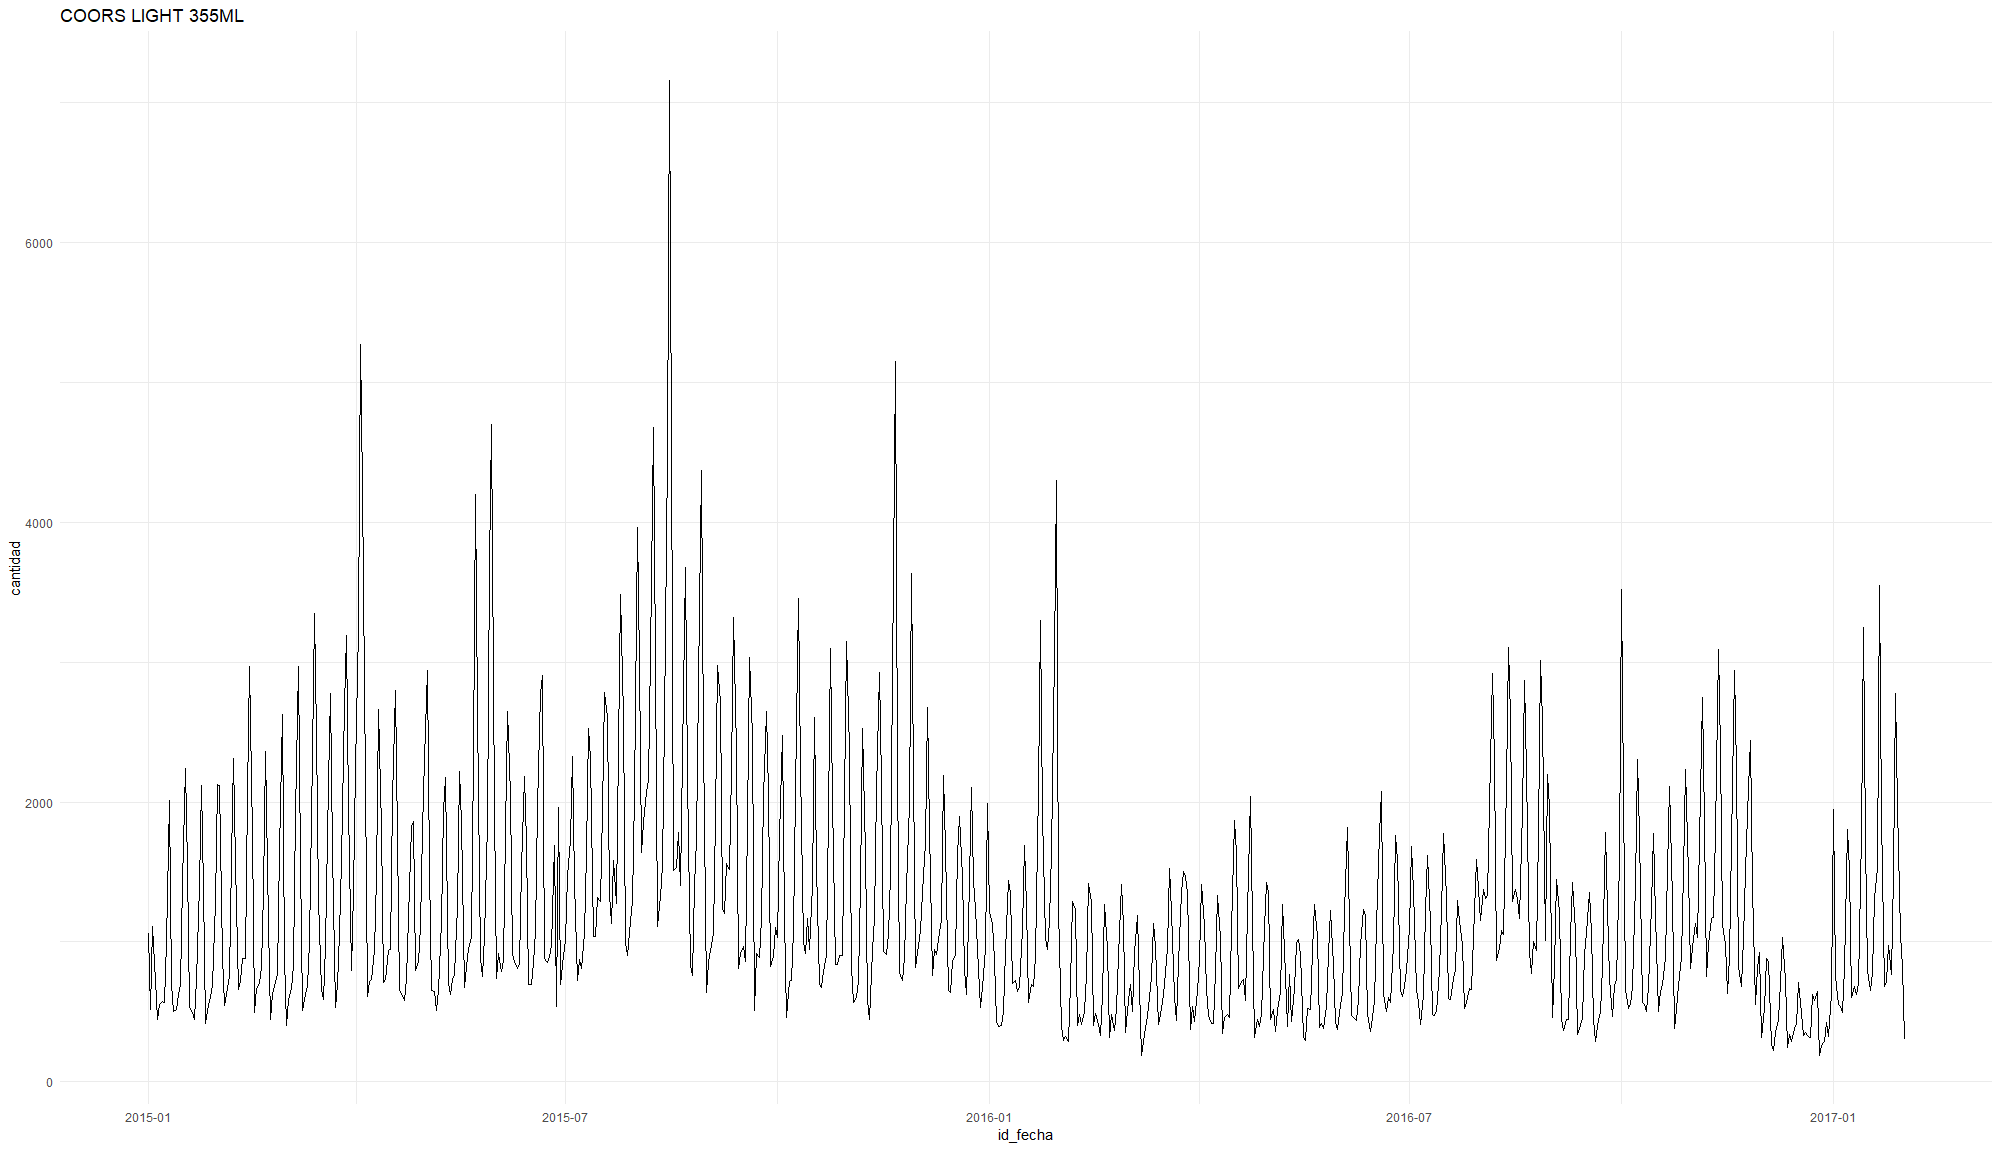
\includegraphics[width=15cm]{1.png}}
\caption{Distribución espacial de las estaciones reportadas (izquierda) y distribución de la precipitación promedio registrada (derecha).}
\label{img1}
\end{figure}
\FloatBarrier   



  \item Identifica la región de interés, el dise\~no, la respuesta y las covariables, si las hay.\\
  
 

En la figura 1.1 ( izquierda) podemos visualizar la región de interés junto con la ubicaciones de las estaciones que se reportan (puntos verdes). Como comentamos en párrafos anteriores el diseño parece apropiado, a primera vista, pues las estaciones aparentan cubrir el estado homogéneamente (aunque una prueba de hipótesis que sustenta lo anterior sería interesante). \\
El conjunto de datos Paraná solo dispone de las coordenadas de las estaciones, los bordes necesarios para visualizar el estado y un registro de las precipitaciones promedio, no se identifican otras covariables. En la figura 1.2 (izquierda) podemos visualizar el conjunto de coordenadas y la precipitación que se registra en los puntos, también en la figura 1.2 (centro y derecha respectivamente) podemos visualizar la precipitación promedio a lo largo de cada una de las coordenadas, es de notar la tendencia a la baja de la precipitación registrada en la dirección noreste del estado de Paraná.


\begin{figure}[htbp]
\center{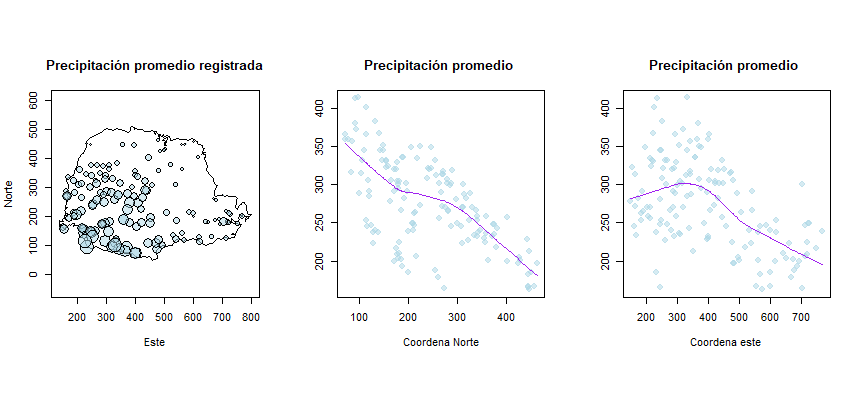
\includegraphics[width=15cm]{2.png}}
\caption{Precipitación promedio (derecha) registrada en cada estación el tamaño de los puntos indica el valor de la variable precipitación. Precipitación en cada coordenada (centro y derecha).}
\label{img1}
\end{figure}
\FloatBarrier   


  \item ¿Cuál es la \emph{señal} subyacente?\\
  Como ya lo hemos comentado, la señal que registran los datos la consideramos como la precipitación promedio en el estado de Paraná en una ventana de tiempo (este aspecto es importante porque acota temporalmente el estudio y la inferencia que podría formarse) que desconocemos.
  \end{enumerate}

El código con el que genera las figuras de esta sección lo anexo en el script \textit{tarea4CD2\_ejercicio1.R}
 
 
\item Considera los siguientes dos modelos para un conjunto de respuestas $Y_i$, $i=1,\ldots,n$, asociados con una secuencia de posiciones $x_i$ a lo largo de un eje espacial de una dimensión $x$.
  \begin{enumerate}
  \item $Y_i=\alpha+\beta x_i + \epsilon_i$, donde $\alpha$ y $\beta$ son parámetros y los $\epsilon_i$ son mutuamente independientes con media cero y varianza $\sigma^2_{\epsilon}$.\\
  
  Encuentra el promedio y varianza de $Y_i$, y la covarianza entre $Y_i$, $Y_j$, para cualquier $j\neq i$.\\\\
   Utilizando la linealidad de la esperanza $E(Y_i) = E(\alpha +\beta x_i + \epsilon_i)=E(\alpha+ \beta x_i) + E(\epsilon_i)$, donde la última igualdad se tiene porque en este caso los parámetros de la regresión son \textit{constantes} al igual que la realización $x_i$, adémas el error tiene media cero tenemos que $E(Y_i)= \alpha + \beta x_i$.\\
  De igual manera como el término $\alpha + \beta x_i$ es constante entonces $V(Y_i)=V(\alpha + \beta x_i + \epsilon_i)= V(\epsilon_i) = \sigma^2_\epsilon$.  \\
  Ahorra para calcular la covarianza entre dos observaciones del modelo anterior recordemos que $\alpha + \beta x_k$ con $ k\in \{i,j\}$ es contante por lo que $Cov(Y_i,Y_j)=Cov(\alpha +\beta x_i + \epsilon_i, \alpha +\beta x_j+ \epsilon_j) = Cov(\epsilon_i, \alpha + \beta x_j +\epsilon_j) = Cov(\epsilon_i, \epsilon_j)$, y como tenemos independencia entre los errores su covarianza es cero, por lo que tenemos que $Cov(Y_i,Y_j)=0$.\\
  

  \item $Y_i=A+Bx_i + \epsilon_i$, donde los $\epsilon_i$ son como en el inciso anterior pero $A$ y $B$ son variables aleatorias, independientes entre sí y entre los $\epsilon_i$, cada una con media cero y varianzas $\sigma^2_{A}$ y $\sigma^2_{B}$. 
  
    Encuentra el promedio y varianza de $Y_i$, y la covarianza entre $Y_i$, $Y_j$, para cualquier $j\neq i$.\\
 
Por la linealidad de la esperanza tenemos que $E(Y_i)=E(A+Bx_i + \epsilon_i)=E(A) + E(B)x_i +E(\epsilon_i)$, y por hipótesis las tres esperanzas anteriores valen cero entonces $E(Y_i)=0$
  
    Al considerar que $A$, $B$ y $\epsilon_i$ son independientes entre si y que $x_i$ es una realización fija tenemos que $V(Y_i)=V(A)+V(Bx_i) + V(\epsilon_i) = \sigma_A^2 + V(B)x_i^2 + \sigma_\epsilon^2=\sigma_A^2+\sigma_B^2x_i^2+\sigma_\epsilon^2$\\

Para terminar este apartado recordemos que en una suma de v.a. independientes cualquier asociación por pares mantiene la independencia, entonces 
\begin{equation*} 
\begin{split}
Cov(Y_i, Y_j) &=Cov(A+Bx_i + \epsilon_i, A+Bx_j + \epsilon_j)=Cov((A+Bx_i )+ \epsilon_i, (A+Bx_j) + \epsilon_j)  \\
 & =Cov(A+Bx_i , (A+Bx_j) + \epsilon_j) + Cov( \epsilon_i, (A+Bx_j) +\epsilon_j) \\
 &=  Cov(A+Bx_i , (A+Bx_j) + \epsilon_j) + Cov( \epsilon_i, (A+Bx_j) ) +Cov( \epsilon_i, \epsilon_j) \\
\end{split}
\end{equation*}
Como $\epsilon_i$ es independiente a $A + Bx_j$ su covarianza es cero, también por hipótesis $\epsilon_i,\epsilon_j$ son independientes por lo que su covarianza es cero, por lo que la expresión anterior se simplifica a:

\begin{equation*} 
\begin{split}
Cov(Y_i, Y_j) =& Cov(A+Bx_i , (A+Bx_j) + \epsilon_j) =  Cov(A+Bx_i , (A+Bx_j) ) + Cov(A+Bx_i , \epsilon_j)\\
\end{split}
\end{equation*}

Nuevamente como la $Cov(A+Bx_i, \epsilon_j)$ es cero (por la independencia de los errores y $A,B$, lo anterior se reduce a: 

\begin{equation*} 
\begin{split}
Cov(Y_i, Y_j) =&   Cov(A+Bx_i  , A+Bx_j ) = Cov(A , A+Bx_j ) + Cov(Bx_i, A+ Bx_j)\\
  & =  Cov(A, A) + Cov(A, Bx_j)+Cov(Bx_i,A)+Cov(Bx_i,Bx_j)
\\
\end{split}
\end{equation*}
Nuevamente aprovechando la independencia entre $A$ y $B$ tenemos que:

$$Cov(Y_i,Y_j)=Cov(A,A)+Cov(Bx_i,Bx_j)=\sigma_A^2+Cov(B, B)x_ix_j=\sigma_A^2+\sigma_B^2x_ix_j$$

Dado una sola realización de cualquier modelo, ¿sería posible distinguirlos?\\\\
Con una sola realización no es posible identificar a los modelos, en el caso de los parámetros fijos tenemos un grado de libertad (suponiendo conocida la varianza de los errores) y en el otro caso con una sola realización sólo distinguiremos (a lo más) un nivel lo cual también tiene un grado de libertad al tener una realización fija. Además con una sola realización no podemos estimar la varianza de ambos modelos que como son diferentes podría dar un indicio de que se trata de dos modelos diferentes, pero sería una estimación poco confiable.



\end{enumerate}


\item Un estudio piloto para estudiar la obesidad infantil fue llevado a cabo en algunas escuelas de los municipios de San Pedro y Santa Catarina en el estado de Nuevo León.\\
  En este estudio, se recopilaron datos a través de encuestas sobre las características familiares y demográficas de ni\~nos en edad preescolar en busca de variables relacionadas con problemas potenciales de obesidad temprana. Luego de un preproceso, que incluyó la georeferenciación de los domicilios, se tienen las ubicaciones.\textbf{ donde se se\~nala con círculos de diferente diámetro, el peso en kilogramos de los ni\~nos.}

  La información del estudio se encuentra en \verb|obesidad.zip|, y contiene los archivos vectoriales \verb|ESRI-shapefile|, que puedes bajar en la plataforma del curso.
  

  \begin{enumerate}
  \item Realiza una estimación espacial mediante Kriging usando como variable de interés (por separado): \verb|Peso|, \verb|Tallacms| y \verb|Circintu|. Compara visualmente los resultados y escribe tus comentarios y conclusiones.\\\\

Después de identificar un par de coordenadas duplicadas introducimos un ruido menor a 0.1 en las mismas con la finalidad de no perder la información de las dos observaciones (en vista de que nuestro tamaño de muestra es 81), pues estas observaciones repetidas implican problemas en las soluciones y métodos numéricos. Se procedió con el siguiente análisis.\\

En la figura 1.3 presentamos los puntos en los que se realizó la encuesta en los municipios de Santa Catarina y San Pedro si bien en el mapa izquierdo podemos observar la distribución desigual de la muestra, en el mapa derecho podemos ver que la zona cuenta con áreas verdes (punto importante para el siguiente inciso).


\begin{figure}[htbp]
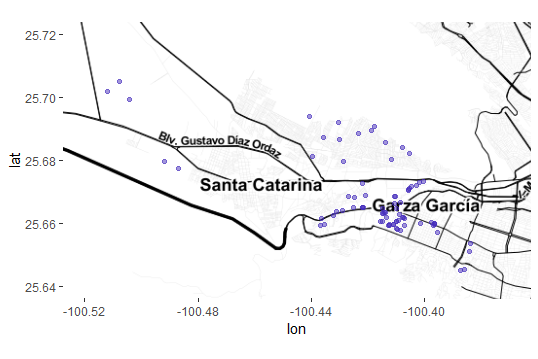
\includegraphics[width=8cm]{mapa1.png}
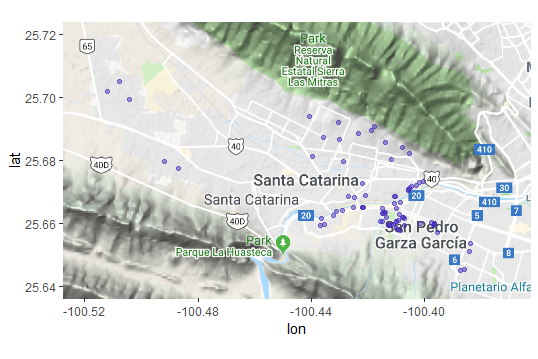
\includegraphics[width=8cm]{mapa2.png}

\caption{Ubicación de los individuos encuestados.}
\label{img1}
\end{figure}
\FloatBarrier     
  
\subsection*{Variable Peso}

En la figura 1.4 ilustramos la distribución espacial así como la distribución en cada coordenada de la variable \textit{Peso}. La distribución de la variable \textit{Peso} es unimodal, no se notan tendencias en ninguna dirección lo que nos facilita el supuesto de homogeneidad intrínseca del proceso no observable que estamos estimando. 

 
  
\begin{figure}[htbp]
\center{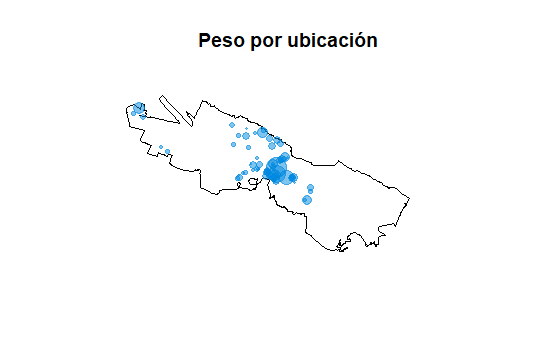
\includegraphics[scale=.7]{peso1.png}}
\center{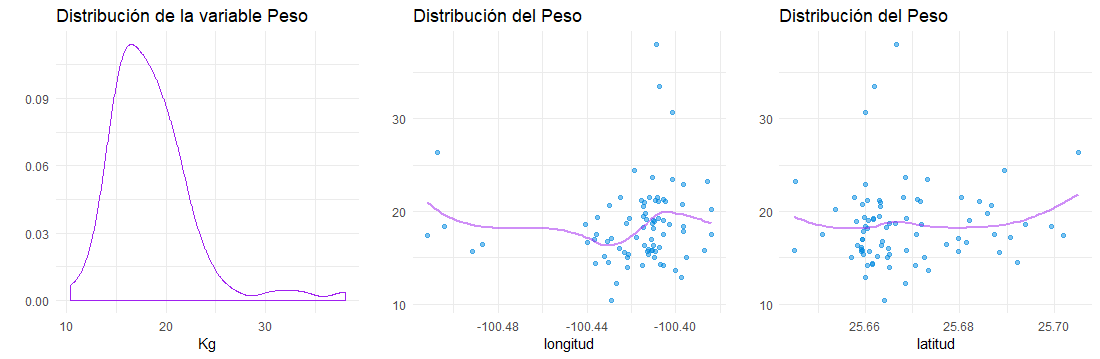
\includegraphics[scale=.5]{peso2.png}}
\caption{Distribución del peso en los municipios de Santa Catarina y San Pedro.}
\label{img1}
\end{figure}
\FloatBarrier
 
Lo curioso de este ejercicio es que el semivariograma (figura 1.5 arriba izquierda) no aumenta en función de la distancia de los puntos, lo que puede apoyar el supuesto de estacionariedad (por que no hay tendencia) o bien que la correlación espacial de nuestro proceso es baja. Es de destacarse que el aumento seguido de un decrecimiento del semivariograma puede deberse a que tenemos dos grupos de observaciones, la mayoría ubicadas en el municipio de San Pedro y unas pocas ubicadas al noroeste de Santa Catarina.  \\

Utilizamos un modelo exponencial para ajustar el semivariograma con kriging ordinario (pues no conocemos la media), sin efecto nugget y con un rango práctico estimado de 0.07091539 y un umbral, o sill, de 25.54907.\\

La interpolación a toda nuestra región de interés se encuentra en la figura 1.5 (arriba derecha) donde se aprecia la homogeneidad de la media en la región de interés, además (figura 1.5 abajo izquierda) la varianza es constante y de poco ‘alcance’ espacial. Concluiría que esta variable es poco informativa en el contexto de geoestadística debido a su baja correlación espacial.



\begin{figure}[htbp]
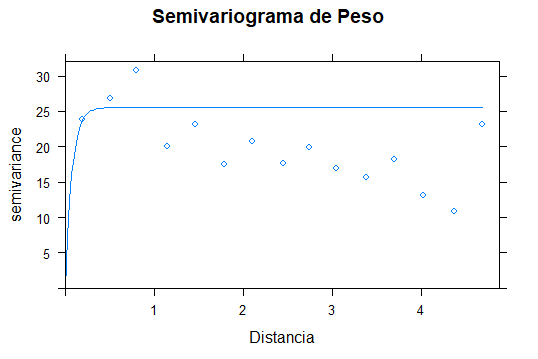
\includegraphics[width=6.5cm]{peso_var.png}
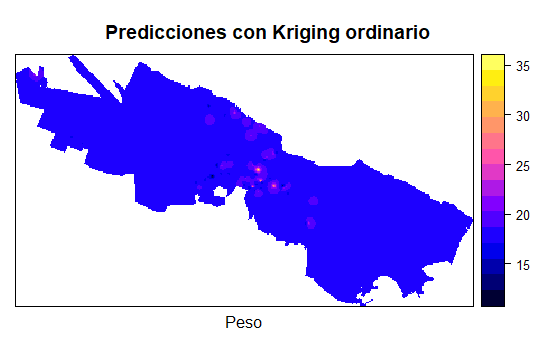
\includegraphics[width=6.5cm]{peso_k1.png}
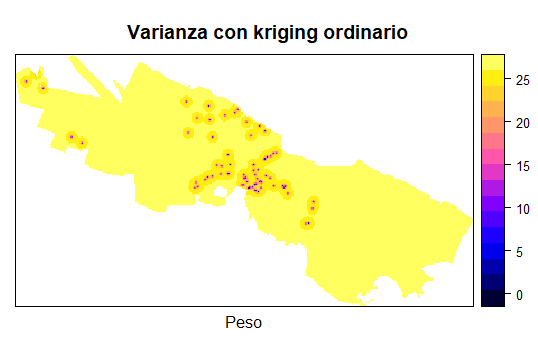
\includegraphics[width=6.5cm]{peso_k2.png}
\caption{Variograma del modelo ajustado (arriba izquierda) para la variable Peso, interpolación a los dos municipio (arriba derecha) y varianzas.}
\label{img1}
\end{figure}
\FloatBarrier     



\subsection*{Variable Talla actual del niño}

La variable que mide la talla del niño en cms resultó de mayor interés espacial que la variable Peso. La figura 1.6 muestra la distribución espacial así como la distribución en cada coordenada de la variable \textit{Talla}. La distribución de la variable \textit{Talla} es unimodal, no se notan tendencias en ninguna dirección sin embargo es importante notar el cambio en la tendencia cuando la señal se registra en los puntos medios de las coordenadas. Sabemos que las muestra se presentan con mayor intensidad en el municipio de San Pedro y esta concentración también presenta una media diferente al resto de la región de estudio.

 
  
\begin{figure}[htbp]
\center{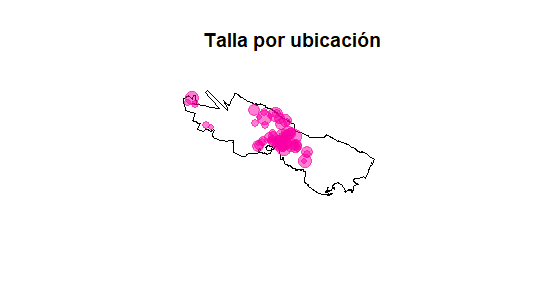
\includegraphics[scale=.8]{talla_ubi.png}}
\center{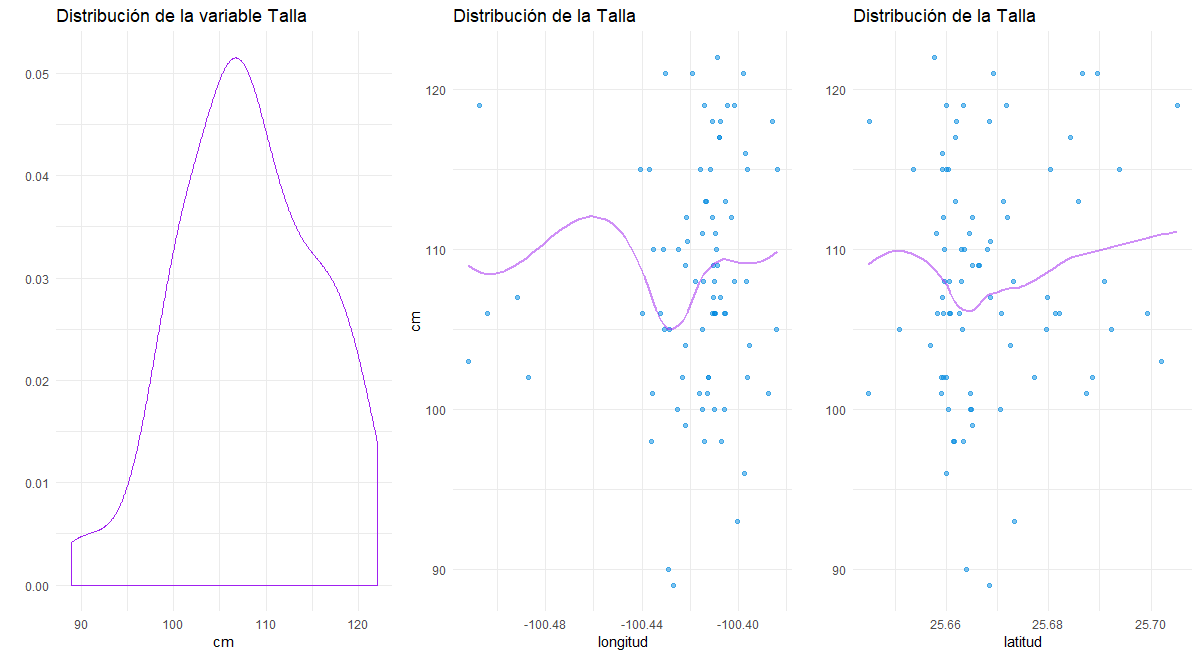
\includegraphics[width=11cm]{talla_distro.png}}
\caption{Distribución de la talla de los niños en los municipios de Santa Catarina y San Pedro.}
\label{img1}
\end{figure}
\FloatBarrier
 
A diferencia del ejercicio anterior el semivariograma de la variable Talla georeferenciada (figura 1.7 arriba izquierda) sí aumenta en función de la distancia de los puntos, pero al parecer después de dos unidades se llega al rango práctico.\\

Ajustamos al semivariograma un modelo esférico en respuesta al cambio de tendencia cuando las observaciones se encuentran cerca de San Pedro (además consideramos este cambio lo suficientemente abrupto como para incluir en la estimación el efecto nugget) utilizando kriging ordinario (pues no conocemos la media), con un nuget de 44, un rango práctico estimado de 2.46 y un umbral, o sill, de 15.82.\\

La interpolación considerando la variable Talla a toda nuestra región de interés se encuentra en la figura 1.7 (arriba derecha) donde se aprecia la no homogeneidad de la media en la región de interés, es interesante el aumento de la estimación en la región centro y más aún en las fronteras al noroeste de la región de estudio además (figura 1.7 abajo izquierda) la varianza disminuye en el centro de la región y presenta un considerable ‘alcance’ espacial. Concluiría que esta variable es informativa en el contexto de geoestadística debido a su peculiar comportamiento al centro de la región de estudio.



\begin{figure}[htbp]
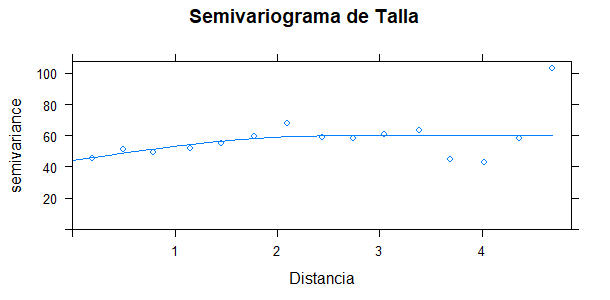
\includegraphics[width=7.5cm]{talla_semivariograma.png}
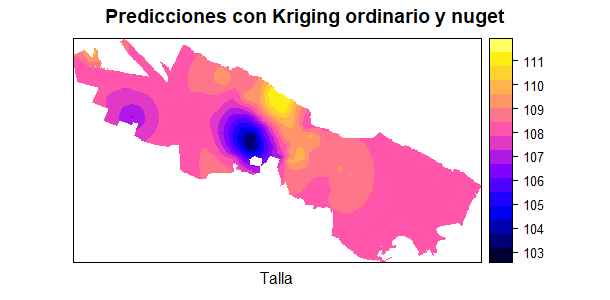
\includegraphics[width=8cm]{talla_predict.png}
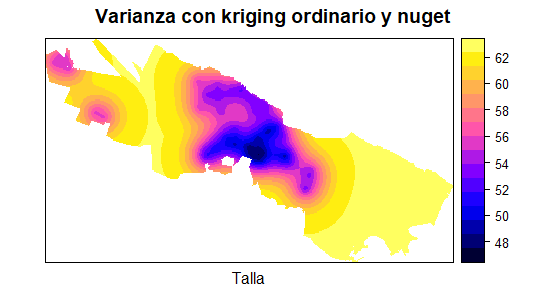
\includegraphics[width=7cm]{talla_varianza.png}
\caption{Variograma del modelo ajustado (arriba izquierda) para la variable Talla, interpolación a los dos municipio (arriba derecha) y varianzas.}
\label{img1}
\end{figure}
\FloatBarrier

\subsection*{Variable Circunferencia cintura}


La variable que mide la circunferencia de la cintura del niño resultó ser la variable más dificíl de ajustar. La figura 1.8 (arriba) muestra la distribución espacial así como la distribución en cada coordenada (abajo) de la variable \textit{Circintu}. La distribución de la variable es unimodal y parece tener menor disperción que las dos variables anteriores, no se notan tendencias en ninguna dirección sin embargo es importante notar al igual que en la variable \textit{Peso} el cambio en la tendencia cuando la señal se registra en los puntos medios de las coordenadas de longitud sugieren un efecto de nuget. \\
 
\begin{figure}[htbp]
\center{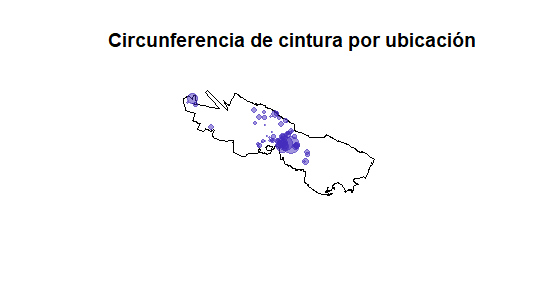
\includegraphics[scale=.8]{circ_ubic.png}}
\center{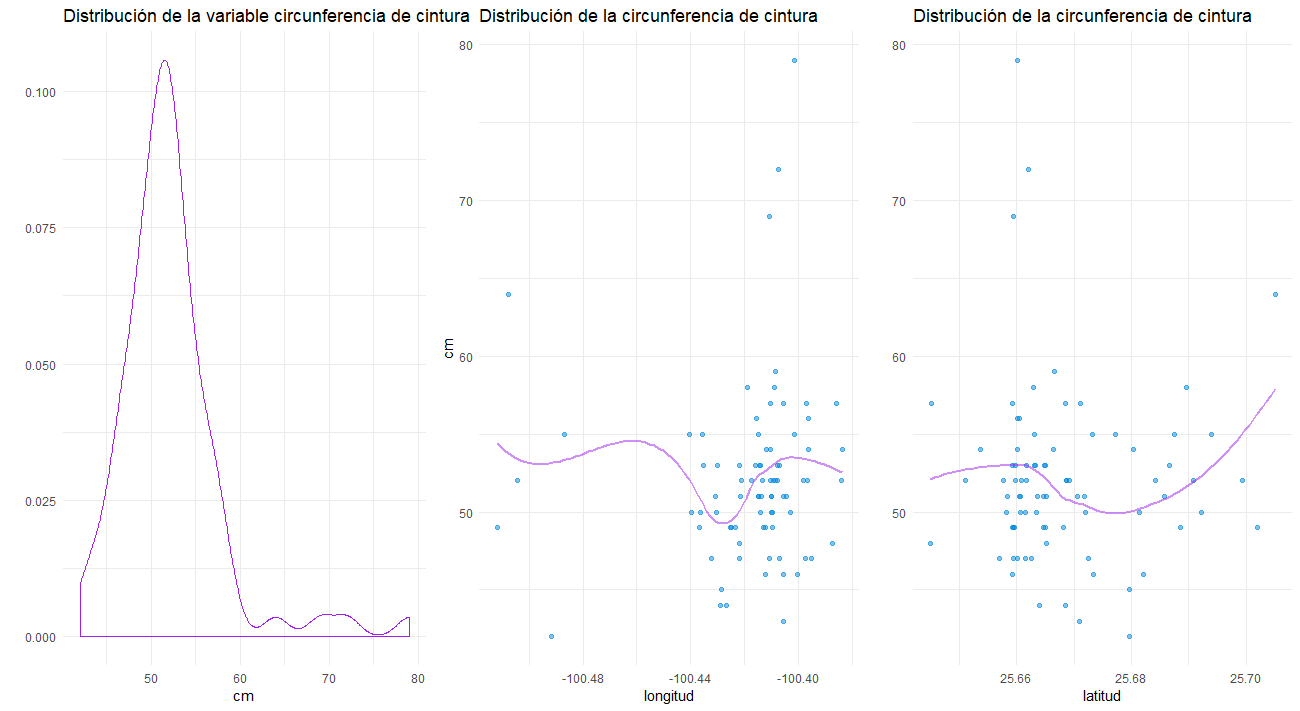
\includegraphics[width=11cm]{circ_distro.png}}
\caption{Distribución de la circunferencia de la cintura de los niños en los municipios de Santa Catarina y San Pedro.}
\label{img1}
\end{figure}
\FloatBarrier
 
 Al igual que con la variable $Peso$ el semivariograma sugiere que la correlación espacial es despreciable pues esta desciende rápidamente en función de la distancia, después de numerosos intentos para ajustar un modelo con nugget (sugerido por el cambio en tendencia a lo largo de la longitud) el modelo ajustado es uno esférico (al igual que en el caso de la variable $Talla$) sin nugget con un rango práctico estimado de 0.3063 y un sill de 37.79 como lo podemos ver en la figura 1.9 (arriba izquierda).\\

Finalmente interpolación considerando la variable $Circintu$ a toda nuestra región de interés se encuentra en la figura 1.9 (arriba derecha) donde se aprecia la homogeneidad de la media en la región de interés a excepción de puntos muy localizados, pese a nuestra intución no encontramos indicios de efecto nuget o anisotropía. En la figura 1.9 (abajo izquierda) la varianza es alta pero homogenéa en la región. Concluiría que esta variable es poco informativa en el contexto de geoestadística.



\begin{figure}[htbp]
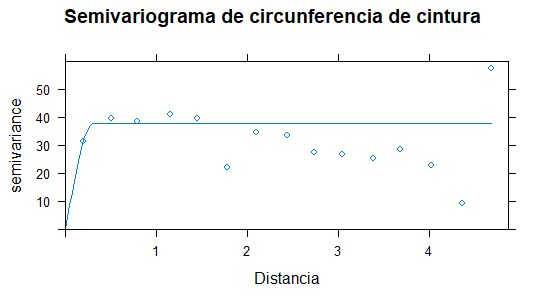
\includegraphics[width=7.5cm]{circ_variograma.png}
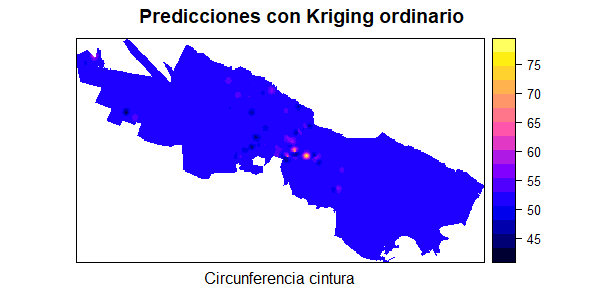
\includegraphics[width=8cm]{circ_predict.png}
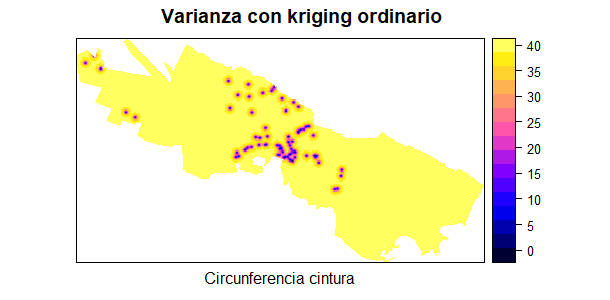
\includegraphics[width=7cm]{circ_varianzas.png}
\caption{Variograma del modelo ajustado (arriba izquierda) para la variable Talla, interpolación a los dos municipio (arriba derecha) y varianzas.}
\label{img1}
\end{figure}
\FloatBarrier





  





  

  
  \item Si el objetivo del estudio es analizar y caracterizar el fenómeno del aumento de peso infantil (no precisamente obesidad) en la región metropolitana de Monterrey, ¿qué tipo de información (de preferencia de acceso libre) sugerirías que se incorporara para tal objetivo?.\\
  En vista de que la muestra parece ser poco informativa por su diseño e implementación y para utilizar estos mismos datos propondría incluir la localización de parques y centros para realizar ejercicio además de la georeferenciación de tiendas de conveniencia y establecimientos que provean de alimentos con alto contenido calórico.\\

Por ejemplo tomemos la ubicación de la primer observación de la encuesta, la cual mostramos en la figura 1.10, podemos notar la presencia de un parque e inclusive un gimnasio. Aunque no parece una tarea fácil es plausible incorporar estas localizaciones para definir una variable continua como ‘distancia de la casa donde habita el niño a un parque’, o bien con la georreferencia de los parques se podrían crear variables dummies que ayudan a estratificar el área de estudio, esto último también favorece a las estimaciones pues actualmente consideramos un solo estrato cuando en los mapas es fácil observar que existen clusters de ubicaciones distantes entre ellos. \\


\begin{figure}[htbp]
\center{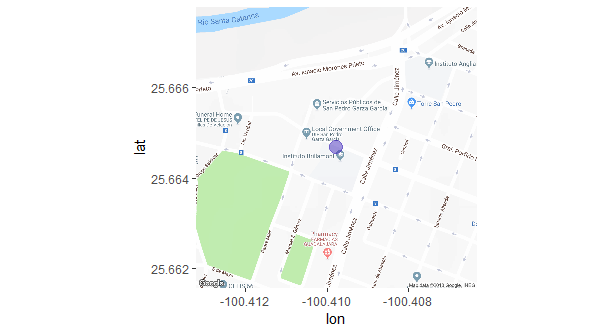
\includegraphics[width=10cm]{mapa_obs1.png}}
\caption{Vecindario de la localización de la primer observación en la encuesta.}
\label{img1}
\end{figure}
\FloatBarrier





  



\end{enumerate}  
\end{enumerate}
\textbf{Notas}
\bigskip

Recuerda que la predicción espacial debe realizarse sobre una región definida. Te sugiero usar la región definida por \verb|poligono_region|. Una pregunta interesante es averiguar qué tanto afecta a la predicción espacial la modificación de la región de interés. Puedes probar usando \verb|poligono_region_mun| ¿Qué tanto cambia respecto a \verb|poligono_region|?
El código con el que se realizaron las estimaciones y visualizaciones del ejercicio 3 se anexan en el script ‘tarea 4 CD2 ejercicio 3.R’. Lo siguiente es una réplica del mismo script cambiando el polígono, y por ende el grid de la región (anexo en el script ‘Extra.R’). \\

De manera rápida realizamos las estimaciones de los semivariogramas de las tres variables de la misma manera, lo que cambiamos fue el grid (si bien este cambio permitiría una nuevo ajuste para cada variable por cuestiones de tiempo nos limitamos a ‘extrapolar’ sobre otra región.\\
En la figura 1.11 se muestran las observaciones georeferenciadas sobre el polígono mencionado, en los tres casos se realizó la regresión con Kriging y podemos distinguir 2 hechos importantes: primero la señal se comporta como isotrópica y estacionaria para distancia grandes (lo cual es natural por la construcción del Kriging, que es un promedio ponderado de las señales observadas), lo anterior nos permite fijar la idea de que Kriging es un método de interpolación y debe de cuidarse de extrapolar con él, ese mismo detalle acota el alcance del modelo pues aunque Kriging es óptimo como interpolador no lo es para la predicción.\\
El segundo aspecto se ve reflejado en la estimación que se realizó para la variable $Talla$pues ampliando el polígono de interés, el efecto de las aristas o fronteras parece suavizarse. 




\begin{figure}[htbp]
\center{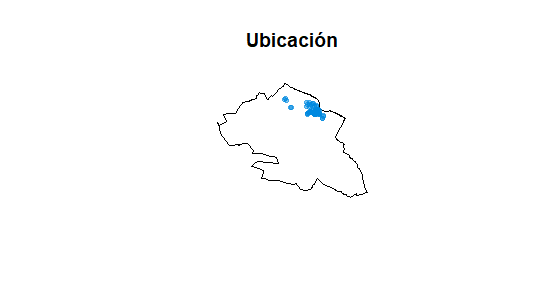
\includegraphics[width=10cm]{big_ubicacion.png}}
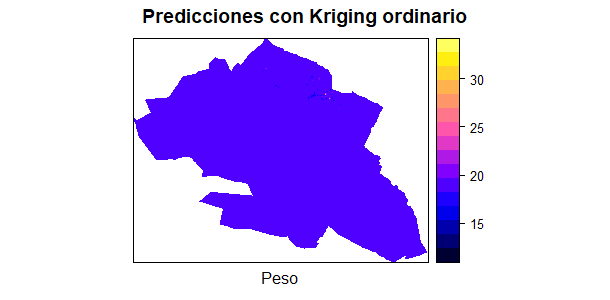
\includegraphics[width=7cm]{big_peso_predict.png}
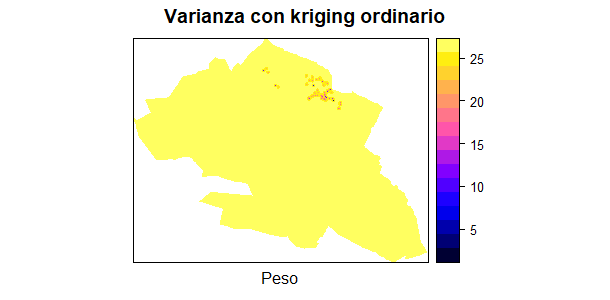
\includegraphics[width=7cm]{big_peso_var.png}
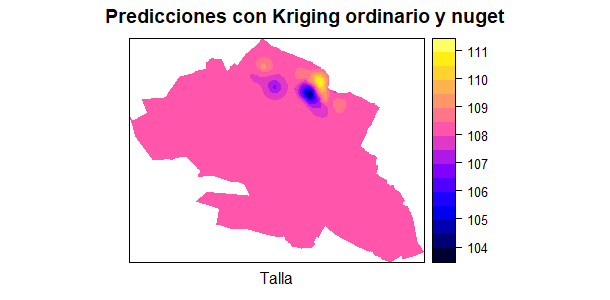
\includegraphics[width=7cm]{big_talla_predict.png}
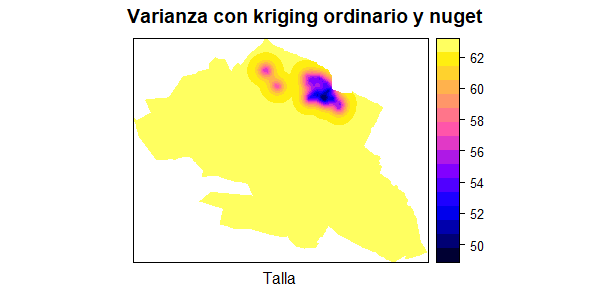
\includegraphics[width=7cm]{big_talla_varianza.png}
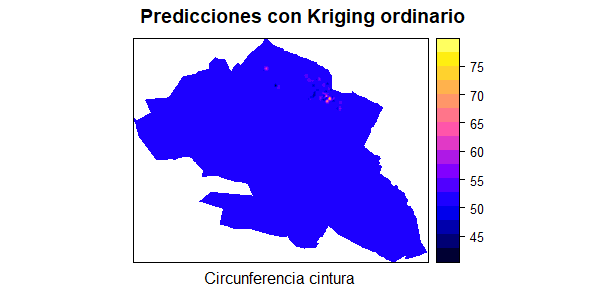
\includegraphics[width=7cm]{big_circ_predict.png}
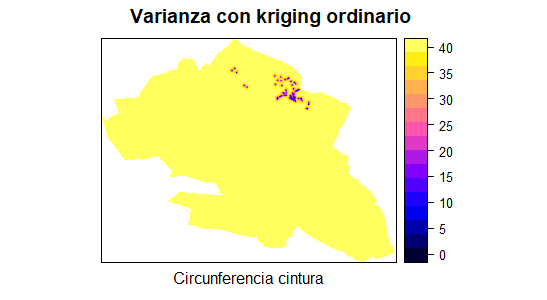
\includegraphics[width=7cm]{big_circ_var.png}

\caption{Interpolación sobre una región de mayor superficie con las mismas observaciones y los mismos modelos.}
\label{img1}
\end{figure}


  
%\begin{thebibliography}{1}
%\bibitem{Hes}
%Hastie T., Tibshirani R. and Friedman J. , \textit{The Elements of Statistical Larning}, Springer 2nd., 2009.

%\end{thebibliography}

\end{document}